\documentclass{article}
\usepackage{iclr2027_conference,times}
%%%%% NEW MATH DEFINITIONS %%%%%

\usepackage{amsmath,amsfonts,bm}

% Mark sections of captions for referring to divisions of figures
\newcommand{\figleft}{{\em (Left)}}
\newcommand{\figcenter}{{\em (Center)}}
\newcommand{\figright}{{\em (Right)}}
\newcommand{\figtop}{{\em (Top)}}
\newcommand{\figbottom}{{\em (Bottom)}}
\newcommand{\captiona}{{\em (a)}}
\newcommand{\captionb}{{\em (b)}}
\newcommand{\captionc}{{\em (c)}}
\newcommand{\captiond}{{\em (d)}}

% Highlight a newly defined term
\newcommand{\newterm}[1]{{\bf #1}}


% Figure reference, lower-case.
\def\figref#1{figure~\ref{#1}}
% Figure reference, capital. For start of sentence
\def\Figref#1{Figure~\ref{#1}}
\def\twofigref#1#2{figures \ref{#1} and \ref{#2}}
\def\quadfigref#1#2#3#4{figures \ref{#1}, \ref{#2}, \ref{#3} and \ref{#4}}
% Section reference, lower-case.
\def\secref#1{section~\ref{#1}}
% Section reference, capital.
\def\Secref#1{Section~\ref{#1}}
% Reference to two sections.
\def\twosecrefs#1#2{sections \ref{#1} and \ref{#2}}
% Reference to three sections.
\def\secrefs#1#2#3{sections \ref{#1}, \ref{#2} and \ref{#3}}
% Reference to an equation, lower-case.
\def\eqref#1{equation~\ref{#1}}
% Reference to an equation, upper case
\def\Eqref#1{Equation~\ref{#1}}
% A raw reference to an equation---avoid using if possible
\def\plaineqref#1{\ref{#1}}
% Reference to a chapter, lower-case.
\def\chapref#1{chapter~\ref{#1}}
% Reference to an equation, upper case.
\def\Chapref#1{Chapter~\ref{#1}}
% Reference to a range of chapters
\def\rangechapref#1#2{chapters\ref{#1}--\ref{#2}}
% Reference to an algorithm, lower-case.
\def\algref#1{algorithm~\ref{#1}}
% Reference to an algorithm, upper case.
\def\Algref#1{Algorithm~\ref{#1}}
\def\twoalgref#1#2{algorithms \ref{#1} and \ref{#2}}
\def\Twoalgref#1#2{Algorithms \ref{#1} and \ref{#2}}
% Reference to a part, lower case
\def\partref#1{part~\ref{#1}}
% Reference to a part, upper case
\def\Partref#1{Part~\ref{#1}}
\def\twopartref#1#2{parts \ref{#1} and \ref{#2}}

\def\ceil#1{\lceil #1 \rceil}
\def\floor#1{\lfloor #1 \rfloor}
\def\1{\bm{1}}
\newcommand{\train}{\mathcal{D}}
\newcommand{\valid}{\mathcal{D_{\mathrm{valid}}}}
\newcommand{\test}{\mathcal{D_{\mathrm{test}}}}

\def\eps{{\epsilon}}


% Random variables
\def\reta{{\textnormal{$\eta$}}}
\def\ra{{\textnormal{a}}}
\def\rb{{\textnormal{b}}}
\def\rc{{\textnormal{c}}}
\def\rd{{\textnormal{d}}}
\def\re{{\textnormal{e}}}
\def\rf{{\textnormal{f}}}
\def\rg{{\textnormal{g}}}
\def\rh{{\textnormal{h}}}
\def\ri{{\textnormal{i}}}
\def\rj{{\textnormal{j}}}
\def\rk{{\textnormal{k}}}
\def\rl{{\textnormal{l}}}
% rm is already a command, just don't name any random variables m
\def\rn{{\textnormal{n}}}
\def\ro{{\textnormal{o}}}
\def\rp{{\textnormal{p}}}
\def\rq{{\textnormal{q}}}
\def\rr{{\textnormal{r}}}
\def\rs{{\textnormal{s}}}
\def\rt{{\textnormal{t}}}
\def\ru{{\textnormal{u}}}
\def\rv{{\textnormal{v}}}
\def\rw{{\textnormal{w}}}
\def\rx{{\textnormal{x}}}
\def\ry{{\textnormal{y}}}
\def\rz{{\textnormal{z}}}

% Random vectors
\def\rvepsilon{{\mathbf{\epsilon}}}
\def\rvtheta{{\mathbf{\theta}}}
\def\rva{{\mathbf{a}}}
\def\rvb{{\mathbf{b}}}
\def\rvc{{\mathbf{c}}}
\def\rvd{{\mathbf{d}}}
\def\rve{{\mathbf{e}}}
\def\rvf{{\mathbf{f}}}
\def\rvg{{\mathbf{g}}}
\def\rvh{{\mathbf{h}}}
\def\rvu{{\mathbf{i}}}
\def\rvj{{\mathbf{j}}}
\def\rvk{{\mathbf{k}}}
\def\rvl{{\mathbf{l}}}
\def\rvm{{\mathbf{m}}}
\def\rvn{{\mathbf{n}}}
\def\rvo{{\mathbf{o}}}
\def\rvp{{\mathbf{p}}}
\def\rvq{{\mathbf{q}}}
\def\rvr{{\mathbf{r}}}
\def\rvs{{\mathbf{s}}}
\def\rvt{{\mathbf{t}}}
\def\rvu{{\mathbf{u}}}
\def\rvv{{\mathbf{v}}}
\def\rvw{{\mathbf{w}}}
\def\rvx{{\mathbf{x}}}
\def\rvy{{\mathbf{y}}}
\def\rvz{{\mathbf{z}}}

% Elements of random vectors
\def\erva{{\textnormal{a}}}
\def\ervb{{\textnormal{b}}}
\def\ervc{{\textnormal{c}}}
\def\ervd{{\textnormal{d}}}
\def\erve{{\textnormal{e}}}
\def\ervf{{\textnormal{f}}}
\def\ervg{{\textnormal{g}}}
\def\ervh{{\textnormal{h}}}
\def\ervi{{\textnormal{i}}}
\def\ervj{{\textnormal{j}}}
\def\ervk{{\textnormal{k}}}
\def\ervl{{\textnormal{l}}}
\def\ervm{{\textnormal{m}}}
\def\ervn{{\textnormal{n}}}
\def\ervo{{\textnormal{o}}}
\def\ervp{{\textnormal{p}}}
\def\ervq{{\textnormal{q}}}
\def\ervr{{\textnormal{r}}}
\def\ervs{{\textnormal{s}}}
\def\ervt{{\textnormal{t}}}
\def\ervu{{\textnormal{u}}}
\def\ervv{{\textnormal{v}}}
\def\ervw{{\textnormal{w}}}
\def\ervx{{\textnormal{x}}}
\def\ervy{{\textnormal{y}}}
\def\ervz{{\textnormal{z}}}

% Random matrices
\def\rmA{{\mathbf{A}}}
\def\rmB{{\mathbf{B}}}
\def\rmC{{\mathbf{C}}}
\def\rmD{{\mathbf{D}}}
\def\rmE{{\mathbf{E}}}
\def\rmF{{\mathbf{F}}}
\def\rmG{{\mathbf{G}}}
\def\rmH{{\mathbf{H}}}
\def\rmI{{\mathbf{I}}}
\def\rmJ{{\mathbf{J}}}
\def\rmK{{\mathbf{K}}}
\def\rmL{{\mathbf{L}}}
\def\rmM{{\mathbf{M}}}
\def\rmN{{\mathbf{N}}}
\def\rmO{{\mathbf{O}}}
\def\rmP{{\mathbf{P}}}
\def\rmQ{{\mathbf{Q}}}
\def\rmR{{\mathbf{R}}}
\def\rmS{{\mathbf{S}}}
\def\rmT{{\mathbf{T}}}
\def\rmU{{\mathbf{U}}}
\def\rmV{{\mathbf{V}}}
\def\rmW{{\mathbf{W}}}
\def\rmX{{\mathbf{X}}}
\def\rmY{{\mathbf{Y}}}
\def\rmZ{{\mathbf{Z}}}

% Elements of random matrices
\def\ermA{{\textnormal{A}}}
\def\ermB{{\textnormal{B}}}
\def\ermC{{\textnormal{C}}}
\def\ermD{{\textnormal{D}}}
\def\ermE{{\textnormal{E}}}
\def\ermF{{\textnormal{F}}}
\def\ermG{{\textnormal{G}}}
\def\ermH{{\textnormal{H}}}
\def\ermI{{\textnormal{I}}}
\def\ermJ{{\textnormal{J}}}
\def\ermK{{\textnormal{K}}}
\def\ermL{{\textnormal{L}}}
\def\ermM{{\textnormal{M}}}
\def\ermN{{\textnormal{N}}}
\def\ermO{{\textnormal{O}}}
\def\ermP{{\textnormal{P}}}
\def\ermQ{{\textnormal{Q}}}
\def\ermR{{\textnormal{R}}}
\def\ermS{{\textnormal{S}}}
\def\ermT{{\textnormal{T}}}
\def\ermU{{\textnormal{U}}}
\def\ermV{{\textnormal{V}}}
\def\ermW{{\textnormal{W}}}
\def\ermX{{\textnormal{X}}}
\def\ermY{{\textnormal{Y}}}
\def\ermZ{{\textnormal{Z}}}

% Vectors
\def\vzero{{\bm{0}}}
\def\vone{{\bm{1}}}
\def\vmu{{\bm{\mu}}}
\def\vtheta{{\bm{\theta}}}
\def\va{{\bm{a}}}
\def\vb{{\bm{b}}}
\def\vc{{\bm{c}}}
\def\vd{{\bm{d}}}
\def\ve{{\bm{e}}}
\def\vf{{\bm{f}}}
\def\vg{{\bm{g}}}
\def\vh{{\bm{h}}}
\def\vi{{\bm{i}}}
\def\vj{{\bm{j}}}
\def\vk{{\bm{k}}}
\def\vl{{\bm{l}}}
\def\vm{{\bm{m}}}
\def\vn{{\bm{n}}}
\def\vo{{\bm{o}}}
\def\vp{{\bm{p}}}
\def\vq{{\bm{q}}}
\def\vr{{\bm{r}}}
\def\vs{{\bm{s}}}
\def\vt{{\bm{t}}}
\def\vu{{\bm{u}}}
\def\vv{{\bm{v}}}
\def\vw{{\bm{w}}}
\def\vx{{\bm{x}}}
\def\vy{{\bm{y}}}
\def\vz{{\bm{z}}}

% Elements of vectors
\def\evalpha{{\alpha}}
\def\evbeta{{\beta}}
\def\evepsilon{{\epsilon}}
\def\evlambda{{\lambda}}
\def\evomega{{\omega}}
\def\evmu{{\mu}}
\def\evpsi{{\psi}}
\def\evsigma{{\sigma}}
\def\evtheta{{\theta}}
\def\eva{{a}}
\def\evb{{b}}
\def\evc{{c}}
\def\evd{{d}}
\def\eve{{e}}
\def\evf{{f}}
\def\evg{{g}}
\def\evh{{h}}
\def\evi{{i}}
\def\evj{{j}}
\def\evk{{k}}
\def\evl{{l}}
\def\evm{{m}}
\def\evn{{n}}
\def\evo{{o}}
\def\evp{{p}}
\def\evq{{q}}
\def\evr{{r}}
\def\evs{{s}}
\def\evt{{t}}
\def\evu{{u}}
\def\evv{{v}}
\def\evw{{w}}
\def\evx{{x}}
\def\evy{{y}}
\def\evz{{z}}

% Matrix
\def\mA{{\bm{A}}}
\def\mB{{\bm{B}}}
\def\mC{{\bm{C}}}
\def\mD{{\bm{D}}}
\def\mE{{\bm{E}}}
\def\mF{{\bm{F}}}
\def\mG{{\bm{G}}}
\def\mH{{\bm{H}}}
\def\mI{{\bm{I}}}
\def\mJ{{\bm{J}}}
\def\mK{{\bm{K}}}
\def\mL{{\bm{L}}}
\def\mM{{\bm{M}}}
\def\mN{{\bm{N}}}
\def\mO{{\bm{O}}}
\def\mP{{\bm{P}}}
\def\mQ{{\bm{Q}}}
\def\mR{{\bm{R}}}
\def\mS{{\bm{S}}}
\def\mT{{\bm{T}}}
\def\mU{{\bm{U}}}
\def\mV{{\bm{V}}}
\def\mW{{\bm{W}}}
\def\mX{{\bm{X}}}
\def\mY{{\bm{Y}}}
\def\mZ{{\bm{Z}}}
\def\mBeta{{\bm{\beta}}}
\def\mPhi{{\bm{\Phi}}}
\def\mLambda{{\bm{\Lambda}}}
\def\mSigma{{\bm{\Sigma}}}

% Tensor
\DeclareMathAlphabet{\mathsfit}{\encodingdefault}{\sfdefault}{m}{sl}
\SetMathAlphabet{\mathsfit}{bold}{\encodingdefault}{\sfdefault}{bx}{n}
\newcommand{\tens}[1]{\bm{\mathsfit{#1}}}
\def\tA{{\tens{A}}}
\def\tB{{\tens{B}}}
\def\tC{{\tens{C}}}
\def\tD{{\tens{D}}}
\def\tE{{\tens{E}}}
\def\tF{{\tens{F}}}
\def\tG{{\tens{G}}}
\def\tH{{\tens{H}}}
\def\tI{{\tens{I}}}
\def\tJ{{\tens{J}}}
\def\tK{{\tens{K}}}
\def\tL{{\tens{L}}}
\def\tM{{\tens{M}}}
\def\tN{{\tens{N}}}
\def\tO{{\tens{O}}}
\def\tP{{\tens{P}}}
\def\tQ{{\tens{Q}}}
\def\tR{{\tens{R}}}
\def\tS{{\tens{S}}}
\def\tT{{\tens{T}}}
\def\tU{{\tens{U}}}
\def\tV{{\tens{V}}}
\def\tW{{\tens{W}}}
\def\tX{{\tens{X}}}
\def\tY{{\tens{Y}}}
\def\tZ{{\tens{Z}}}


% Graph
\def\gA{{\mathcal{A}}}
\def\gB{{\mathcal{B}}}
\def\gC{{\mathcal{C}}}
\def\gD{{\mathcal{D}}}
\def\gE{{\mathcal{E}}}
\def\gF{{\mathcal{F}}}
\def\gG{{\mathcal{G}}}
\def\gH{{\mathcal{H}}}
\def\gI{{\mathcal{I}}}
\def\gJ{{\mathcal{J}}}
\def\gK{{\mathcal{K}}}
\def\gL{{\mathcal{L}}}
\def\gM{{\mathcal{M}}}
\def\gN{{\mathcal{N}}}
\def\gO{{\mathcal{O}}}
\def\gP{{\mathcal{P}}}
\def\gQ{{\mathcal{Q}}}
\def\gR{{\mathcal{R}}}
\def\gS{{\mathcal{S}}}
\def\gT{{\mathcal{T}}}
\def\gU{{\mathcal{U}}}
\def\gV{{\mathcal{V}}}
\def\gW{{\mathcal{W}}}
\def\gX{{\mathcal{X}}}
\def\gY{{\mathcal{Y}}}
\def\gZ{{\mathcal{Z}}}

% Sets
\def\sA{{\mathbb{A}}}
\def\sB{{\mathbb{B}}}
\def\sC{{\mathbb{C}}}
\def\sD{{\mathbb{D}}}
% Don't use a set called E, because this would be the same as our symbol
% for expectation.
\def\sF{{\mathbb{F}}}
\def\sG{{\mathbb{G}}}
\def\sH{{\mathbb{H}}}
\def\sI{{\mathbb{I}}}
\def\sJ{{\mathbb{J}}}
\def\sK{{\mathbb{K}}}
\def\sL{{\mathbb{L}}}
\def\sM{{\mathbb{M}}}
\def\sN{{\mathbb{N}}}
\def\sO{{\mathbb{O}}}
\def\sP{{\mathbb{P}}}
\def\sQ{{\mathbb{Q}}}
\def\sR{{\mathbb{R}}}
\def\sS{{\mathbb{S}}}
\def\sT{{\mathbb{T}}}
\def\sU{{\mathbb{U}}}
\def\sV{{\mathbb{V}}}
\def\sW{{\mathbb{W}}}
\def\sX{{\mathbb{X}}}
\def\sY{{\mathbb{Y}}}
\def\sZ{{\mathbb{Z}}}

% Entries of a matrix
\def\emLambda{{\Lambda}}
\def\emA{{A}}
\def\emB{{B}}
\def\emC{{C}}
\def\emD{{D}}
\def\emE{{E}}
\def\emF{{F}}
\def\emG{{G}}
\def\emH{{H}}
\def\emI{{I}}
\def\emJ{{J}}
\def\emK{{K}}
\def\emL{{L}}
\def\emM{{M}}
\def\emN{{N}}
\def\emO{{O}}
\def\emP{{P}}
\def\emQ{{Q}}
\def\emR{{R}}
\def\emS{{S}}
\def\emT{{T}}
\def\emU{{U}}
\def\emV{{V}}
\def\emW{{W}}
\def\emX{{X}}
\def\emY{{Y}}
\def\emZ{{Z}}
\def\emSigma{{\Sigma}}

% entries of a tensor
% Same font as tensor, without \bm wrapper
\newcommand{\etens}[1]{\mathsfit{#1}}
\def\etLambda{{\etens{\Lambda}}}
\def\etA{{\etens{A}}}
\def\etB{{\etens{B}}}
\def\etC{{\etens{C}}}
\def\etD{{\etens{D}}}
\def\etE{{\etens{E}}}
\def\etF{{\etens{F}}}
\def\etG{{\etens{G}}}
\def\etH{{\etens{H}}}
\def\etI{{\etens{I}}}
\def\etJ{{\etens{J}}}
\def\etK{{\etens{K}}}
\def\etL{{\etens{L}}}
\def\etM{{\etens{M}}}
\def\etN{{\etens{N}}}
\def\etO{{\etens{O}}}
\def\etP{{\etens{P}}}
\def\etQ{{\etens{Q}}}
\def\etR{{\etens{R}}}
\def\etS{{\etens{S}}}
\def\etT{{\etens{T}}}
\def\etU{{\etens{U}}}
\def\etV{{\etens{V}}}
\def\etW{{\etens{W}}}
\def\etX{{\etens{X}}}
\def\etY{{\etens{Y}}}
\def\etZ{{\etens{Z}}}

% The true underlying data generating distribution
\newcommand{\pdata}{p_{\rm{data}}}
% The empirical distribution defined by the training set
\newcommand{\ptrain}{\hat{p}_{\rm{data}}}
\newcommand{\Ptrain}{\hat{P}_{\rm{data}}}
% The model distribution
\newcommand{\pmodel}{p_{\rm{model}}}
\newcommand{\Pmodel}{P_{\rm{model}}}
\newcommand{\ptildemodel}{\tilde{p}_{\rm{model}}}
% Stochastic autoencoder distributions
\newcommand{\pencode}{p_{\rm{encoder}}}
\newcommand{\pdecode}{p_{\rm{decoder}}}
\newcommand{\precons}{p_{\rm{reconstruct}}}

\newcommand{\laplace}{\mathrm{Laplace}} % Laplace distribution

\newcommand{\E}{\mathbb{E}}
\newcommand{\Ls}{\mathcal{L}}
\newcommand{\R}{\mathbb{R}}
\newcommand{\emp}{\tilde{p}}
\newcommand{\lr}{\alpha}
\newcommand{\reg}{\lambda}
\newcommand{\rect}{\mathrm{rectifier}}
\newcommand{\softmax}{\mathrm{softmax}}
\newcommand{\sigmoid}{\sigma}
\newcommand{\softplus}{\zeta}
\newcommand{\KL}{D_{\mathrm{KL}}}
\newcommand{\Var}{\mathrm{Var}}
\newcommand{\standarderror}{\mathrm{SE}}
\newcommand{\Cov}{\mathrm{Cov}}
% Wolfram Mathworld says $L^2$ is for function spaces and $\ell^2$ is for vectors
% But then they seem to use $L^2$ for vectors throughout the site, and so does
% wikipedia.
\newcommand{\normlzero}{L^0}
\newcommand{\normlone}{L^1}
\newcommand{\normltwo}{L^2}
\newcommand{\normlp}{L^p}
\newcommand{\normmax}{L^\infty}

\newcommand{\parents}{Pa} % See usage in notation.tex. Chosen to match Daphne's book.

\DeclareMathOperator*{\argmax}{arg\,max}
\DeclareMathOperator*{\argmin}{arg\,min}

\DeclareMathOperator{\sign}{sign}
\DeclareMathOperator{\Tr}{Tr}
\let\ab\allowbreak

\usepackage[hidelinks]{hyperref}
\usepackage{url}
\usepackage{graphicx}
\usepackage{booktabs}
\usepackage{amsmath,amssymb}
\usepackage{xcolor}
\usepackage{tabularx}
\usepackage{multirow}
\usepackage{enumitem}
\makeatletter\let\tabinput\@@input\makeatother
\setlist{nosep,leftmargin=*}

\title{Unlearnable Text for LLM Fine-Tuning:\\ Min--Min Word Swaps Fail, a One-Character Hint Works}

\author{Aryan Patyal \& Arjun Korath\\
School of Computing and Augmented Intelligence, Arizona State University\\
CSE 472 Social Media Mining, Project 2.5 \quad Mentor: Chengshuai Zhao}

\iclrfinalcopy
\begin{document}
\maketitle

\begin{abstract}
People publish text that is later scraped to fine-tune large language models (LLMs) without their consent.
\emph{Unlearnable examples} modify data before release so that a model trained on it learns a useless shortcut instead of
the content. We ask whether the error-minimizing (min--min) formulation of \citet{huang2021unlearnable}, adapted to
text by \citet{li2023maketext}, protects a question-answering dataset against LoRA fine-tuning of 8B-parameter LLMs.
We extend it with an answer-letter loss, a Llama-3-8B + LoRA surrogate and HotFlip-guided whole-word swaps under
meaning and fluency constraints, and evaluate on ARC-Challenge with Llama-3-8B (white-box) and Qwen3-8B (black-box)
victims. \textbf{Answer: no.} Protected data lets Llama-3-8B keep the same share of its fine-tuning gain as random edits
with the same budget (80.03\% vs.\ 80.18\% test accuracy; clean 82.62\%, zero-shot 77.47\%), and swaps from the first
round of the optimization do no better (79.81\%). The surrogate memorizes the edited training text within one round,
and the resulting swaps are example-specific rather than a shared shortcut. In a pre-registered bonus experiment, a
single \texttt{!} appended to the correct choice, with no optimization at all, removes the entire fine-tuning gain on
all three victims in every seed and drives Llama-3-8B to 51.45\%, far below zero-shot.
\end{abstract}

\section{Introduction}
Social media posts, forum answers and personal writing are routinely collected to train and fine-tune LLMs, and the
authors of that text have no say in it. Once text is scraped, after-the-fact remedies such as machine unlearning or
watermark-based detection require the model trainer's cooperation. A data owner's only lever is the text itself,
\emph{before} it is published. Unlearnable examples \citep{huang2021unlearnable,li2025survey} use that lever: they add a
small, human-imperceptible perturbation chosen so that training on the protected data drives the loss to near zero
through a shortcut, leaving the model nothing to learn about the actual content.

This idea has been demonstrated for images \citep{huang2021unlearnable} and for small text classifiers and extractive
QA models \citep{li2023maketext}. Whether it survives the setting that matters most today, parameter-efficient
fine-tuning of billion-parameter pretrained LLMs, is open. \textbf{Research question:} does an LLM adaptation of the
min--min unlearnable-example method keep an attacker who fine-tunes Llama-3-8B or Qwen3-8B on protected ARC-Challenge
questions from gaining accuracy? \textbf{One-sentence answer:} no; it is no better than random word edits, because an 8B
surrogate memorizes its edited training text instead of forming a shortcut, whereas a single consistent marker on the correct
answer does make the data unlearnable for every model we tested.

\textbf{Contributions.} (1) A concrete LLM adaptation of min--min unlearnable text (answer-letter loss, LoRA surrogate,
filtered HotFlip word swaps) with the code and protected data kept in our project repository. (2) A controlled evaluation
with three victims, three seeds, a matched random-edit control and the round-0 variant, showing no protection beyond
random edits. (3) A diagnosis: surrogate memorization and the absence of any label-correlated pattern in the swaps.
(4) A pre-registered bonus showing that a one-character answer hint is a strong, transferable shortcut.

\section{Related Works}
\textbf{Unlearnable examples.} \citet{huang2021unlearnable} formulate unlearnable images as a bilevel problem in which
both the model and a bounded noise $\boldsymbol{\delta}$ minimize the training loss; the resulting \emph{error-minimizing}
noise lets the network fit the training set through the noise alone, so clean test accuracy collapses. They compare
sample-wise and class-wise noise and find class-wise noise especially effective. \citet{li2025survey} survey later work,
and VTG \citep{li2025vtg} trains a single generator for transfer across datasets and architectures.

\textbf{Unlearnable text.} \citet{li2023maketext} adapt min--min to text: the noise becomes word substitutions chosen
by a first-order (HotFlip-style; \citealp{ebrahimi2018hotflip}) estimate of the loss change, constrained to embedding
neighbours with cosine similarity $\ge 0.5$ \citep{alzantot2018generating}, one substitution per example, with LSTM and
BiDAF surrogates. Their key observation is that effective substitutions collapse into \emph{simple patterns}: words that
correlate with the label (in their most effective, round-0 sets, zero Jaccard overlap between classes, and five words
cover 60--100\% of a class's substitutions) or a marker next to the answer span. Hand-made ``label hints'' and ``answer hints'' then protect BERT and RoBERTa fine-tuning without any
optimization. Our bonus is that idea, transplanted to LLM fine-tuning. Mechanistically, all of these exploit
\emph{shortcut learning} \citep{geirhos2020shortcut}.

\textbf{LLMs and pretraining.} TextCloak \citep{zhao2026textcloak} targets LLM fine-tuning directly, training a
reinforcement-learning policy that rewrites text and scoring rewrites with fine-tuned surrogate LLMs; it changes far more
than two words. Its authors argue that a low surrogate training loss need not degrade a fine-tuned LLM, because of the
LLM's pretraining priors, and so reward downstream degradation directly. Their experiments include Li and Liu's
min--min word substitutions as a baseline: on ARC-Challenge, across four LLMs it was not optimized against, it changes
test accuracy by at most 2.6 points. \citet{li2026priors} show, in image classification, that pretrained models can
learn genuine features despite unlearnable shortcuts, which defeats protection designed for models trained from scratch.
Our negative result agrees with both findings, here with our own LLM surrogate and a white-box victim.

\section{Model Description (Design Checkpoint)}\label{sec:method}
\textbf{Threat model.} The defender owns a set of question--answer pairs and may edit the question and choice text
before publishing, but may not change the answer, must keep the text readable, and does not know which model the
attacker will fine-tune. The attacker LoRA-fine-tunes a pretrained LLM on the published data. Protection succeeds if the
attacker's clean-test accuracy stays near the model's zero-shot accuracy.

\textbf{Bilevel objective.} Following \citet{huang2021unlearnable}, with $x_i$ the question plus its choices, $y_i$
the answer letter and $\boldsymbol\delta_i$ a set of word swaps,
\begin{equation}
\min_{\boldsymbol\delta}\;\min_{\theta}\;\sum_{i=1}^{N}\ell_{\text{ans}}\big(f_\theta(x_i\oplus\boldsymbol\delta_i),\,y_i\big)
\quad\text{s.t.}\quad |\boldsymbol\delta_i|\le k,
\end{equation}
together with the meaning and fluency constraints $\text{SBERT}(x_i,x_i\oplus\boldsymbol\delta_i)\ge 0.9$ and
$\text{PPL}_{\text{GPT-2}}(x_i\oplus\boldsymbol\delta_i)\le 1.2\,\text{PPL}_{\text{GPT-2}}(x_i)$.
Both levels \emph{minimize} the loss: the swaps make each example easier to fit, so training extracts little from it.

\textbf{Loss: answer-letter cross-entropy.} The prompt is \texttt{Question: \dots\textbackslash nA. \dots\textbackslash
nB. \dots\textbackslash nAnswer:} and the target is the single token \texttt{\textvisiblespace X}. All prompt tokens are
masked (label $-100$), so $\ell_{\text{ans}}$ is the next-token cross-entropy of the answer letter only.
\emph{Why:} the knowledge we protect is the question$\rightarrow$answer mapping, and the answer letter plays the role of
a class label, which keeps the formulation directly comparable to the classification setting of
\citet{huang2021unlearnable} and \citet{li2023maketext}. The same encoding function drives surrogate training, the
gradient and the exact re-scoring, so the search and training optimize one objective. Long prompts are truncated from
the left so the answer token is never cut.

\textbf{Surrogate: Llama-3-8B + LoRA, with the victim's exact settings.} LoRA \citep{hu2022lora} with $r=16$,
$\alpha=32$, dropout $0.05$ on all seven attention and MLP projections. \emph{Why:} the guideline fixes the surrogate
model; matching the attacker's training recipe makes the white-box case truly white-box and isolates transfer as the
only difference in the black-box case.

\textbf{Perturbation: HotFlip-guided whole-word swaps.} Candidate replacements for each word are its 50 nearest
neighbours in Llama-3-8B's input-embedding space (cosine), restricted to single-token whole words (4{,}350 distinct editable words,
covering about 95\% of the word occurrences in the training questions). The lists were computed from the input
embeddings of the \texttt{NousResearch/Meta-Llama-3-8B} mirror, a re-upload of the same weights. For a word at position
$p$ with embedding $\mathbf e_{\text{old}}$, the loss change from swapping in $\mathbf e_{\text{new}}$ is estimated as
$(\mathbf e_{\text{new}}-\mathbf e_{\text{old}})^\top\nabla_{\mathbf e_p}\ell_{\text{ans}}$. Li and Liu's Eq.~5 scores
$\mathbf e_s^\top\nabla\ell$ only; within one position the two rankings are identical, but only the difference is a
valid first-order estimate across positions, so we use it, as does \citet[Eq.~4]{zhao2026textcloak}. One backward pass
scores every (position, neighbour) pair; we keep the 20 most negative, drop those failing the filters, re-score the
survivors exactly, and accept the best only if it really lowers the loss. This is done greedily up to $k=2$ swaps, with
the gradient recomputed after each. \emph{Why:} whole-word, one-token swaps are the only edits for which the HotFlip
estimate is meaningful, keep token positions fixed, and stay readable. Two swaps per question (rather than Li and Liu's
one) gives the optimizer room on short ARC questions.

\textbf{Meaning filters.} Embedding neighbours mix synonyms with opposites: in an early test the search turned the
correct answer ``dry palms'' into ``moist palms''. We therefore (i) never edit or insert a negation word, (ii) block a
swap if any WordNet \citep{miller1995wordnet} synonym of one word is an antonym of the other (catching
increase$\rightarrow$reduce, larger$\rightarrow$smaller), and (iii) require SBERT similarity $\ge 0.9$
\citep{reimers2019sbert} and GPT-2 perplexity $\le 1.2\times$ the original \citep{radford2019gpt2}, both measured
against the \emph{original} example so they bound all $k$ edits together.

\textbf{Loop and stopping rule.} Round 0 searches swaps against the untrained surrogate (Li and Liu's ``Error-min-0'').
Each round $r\ge1$ trains the surrogate for 2 epochs on round $r{-}1$'s protected set, records its training accuracy,
then searches again starting from the original text. Li and Liu stop when \emph{test} metrics stop changing, which tunes
the protection on the test set; Huang et al.\ stop at high accuracy on the perturbed training data. Because an 8B model
can reach 99\% training accuracy by memorization alone, we disabled early stopping and ran a fixed five rounds, saving
every round.

\textbf{Control.} Random edits use the same editable words, neighbour lists, filters and budget $k=2$, but choose
positions and replacements uniformly at random. If random edits protect as well, the optimization is not contributing.

\section{Experiment}
\subsection{Setup}
\textbf{Data.} ARC-Challenge \citep{clark2018arc}: 1{,}119 train / 299 validation / 1{,}172 test questions (train: 1{,}117
four-choice, one three-choice, one five-choice; numeric labels mapped to letters). We protect the train split and always
evaluate on the clean test split.

\textbf{Models.} Llama-3-8B base \citep{grattafiori2024llama3} is the surrogate and the white-box victim; Qwen3-8B
\citep{yang2025qwen3} is the black-box victim. Because Qwen3-8B turned out to gain little from fine-tuning, we added
Qwen3-8B-Base as a second black-box victim (Section~\ref{sec:analysis}).

\textbf{Fine-tuning (identical for every victim run).} LoRA via \texttt{peft}
\citep{mangrulkar2022peft}: $r=16$, $\alpha=32$, dropout 0.05, targets q/k/v/o/gate/up/down projections; AdamW, learning
rate $10^{-4}$, no weight decay, 5\% linear warm-up then linear decay, gradient clipping 1.0, batch size 8, 3 epochs,
max length 512, bf16, gradient checkpointing; answer-letter loss as in Section~\ref{sec:method}. The surrogate uses the
same settings except that it trains 2 epochs per min--min round.

\textbf{Evaluation.} Accuracy on the clean test set, predicting the letter with the highest next-token logit among the
letters that question actually has (no free generation). Seeds 1--3 for every fine-tune; we report mean $\pm$ sample
standard deviation, and compare conditions with Welch's $t$-test over seeds \citep{virtanen2020scipy}. Readability: mean GPT-2 perplexity of question+choices (absolute, and the mean per-question ratio to
the original). Meaning: mean SBERT (\texttt{all-MiniLM-L6-v2}; \citealp{wang2020minilm}) cosine similarity to the
original text.

\textbf{Compute.} One NVIDIA A100 (80 GB) per job on ASU's Sol supercomputer \citep{jennewein2023sol}. Protection (six
searches and five surrogate trainings) took one job; each victim fine-tune took about three minutes.

\subsection{Results (Results Checkpoint)}
Table~\ref{tab:main} is the guideline's results table, extended with the round-0 set, the bonus and the third victim.
Figure~\ref{fig:tradeoff} plots each training set's test accuracy against its meaning preservation.

\begin{table}[t]
\caption{Clean ARC-Challenge test accuracy (\%) after LoRA fine-tuning on each training set (mean $\pm$ std over 3
seeds; lower = stronger protection), with the readability and meaning of that training text. Perplexity: mean GPT-2 perplexity (mean per-question
ratio to the original in brackets). The edit statistics are properties of the training data, so they are the same for
every victim. Random-edit readability was measured once on the same file.}
\label{tab:main}
\vspace{2pt}\centering\small
\begin{tabular}{llccc}
\toprule
Victim & Training data & Test acc.\ (\%) & GPT-2 PPL (ratio) & SBERT \\
\midrule
\tabinput table_main.tex
\bottomrule
\end{tabular}
\end{table}

\begin{figure}[t]
\centering
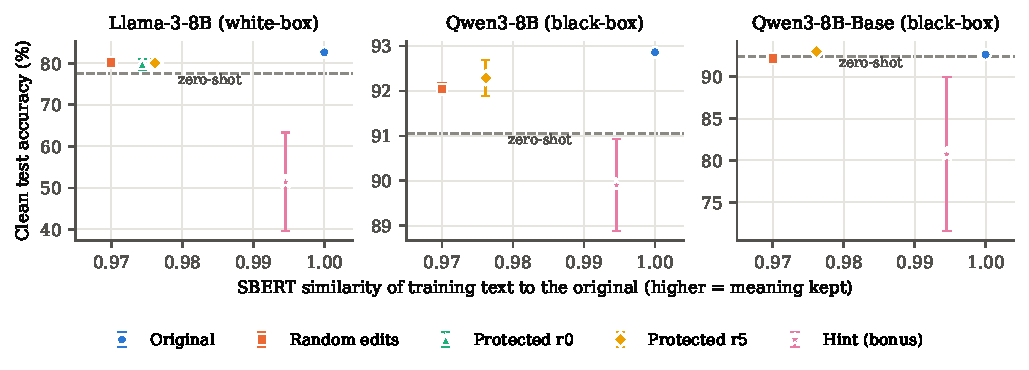
\includegraphics[width=\linewidth]{figures/tradeoff.pdf}
\caption{Protection vs.\ meaning trade-off. Each point is one training set (mean $\pm$ std over 3 seeds); the dashed
line is the victim's zero-shot accuracy. Good protection sits at the bottom right: low accuracy while keeping the
meaning. Min--min protected sets (r0, r5) sit beside random edits; the one-character hint sits at the bottom right.}
\label{fig:tradeoff}
\end{figure}

\textbf{Reference points.} Fine-tuning on the original data raises Llama-3-8B from 77.47\% to 82.62\% (+5.15 points),
the headroom any protection must remove. Qwen3-8B gains only +1.82 (91.04$\rightarrow$92.86) and Qwen3-8B-Base +0.23
(92.41$\rightarrow$92.63).

\textbf{White-box (Llama-3-8B).} The final protected set gives 80.03 $\pm$ 0.92, within seed noise of random edits
(80.18 $\pm$ 0.50) and of the round-0 set (79.81 $\pm$ 1.30): the differences are smaller than one standard deviation
(protected vs.\ random $p=0.83$, round 0 vs.\ random $p=0.68$), while every edited set is clearly below clean
fine-tuning (protected vs.\ clean $p=0.02$, random vs.\ clean $p=0.005$). With three seeds the test has little power,
so this shows no detectable difference, not proof of none. All three edited sets remove about half the fine-tuning
gain, but optimization adds nothing detectable beyond the damage any two word swaps do.

\textbf{Black-box (Qwen3-8B, Qwen3-8B-Base).} Protected and random sets stay within one point of each other and of
clean fine-tuning (Qwen3-8B: 92.29 vs.\ 92.04 vs.\ 92.86). With under two points of headroom these victims cannot
separate the two, so the white-box result is the decisive one.

\textbf{Readability and meaning.} The protected sets are slightly \emph{more} fluent and faithful than random edits
(SBERT 0.976 vs.\ 0.970; PPL ratio 1.08 vs.\ 1.13), because they make fewer edits (1.18 vs.\ 1.87 per question): the
search only accepts a swap that lowers the loss, and 21\% of questions got none.

\textbf{Surrogate.} Figure~\ref{fig:rounds} shows the surrogate's answer loss on clean and protected training questions.
The protected loss falls to 0.0068 by round 5 (clean: 0.213), so the optimization succeeds on its own objective, while
the surrogate's accuracy on the protected set is 99.2\% after the first round and $\ge$99.7\% afterwards. Its loss on the
unedited versions of the same questions stays at 0.21--0.54 in rounds 1--5, so what it fits is the edited text, not the
questions themselves.

\begin{figure}[t]
\centering
\begin{minipage}[t]{0.46\linewidth}\vspace{0pt}
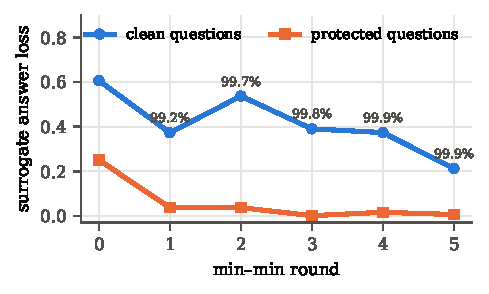
\includegraphics[width=\linewidth]{figures/rounds.pdf}
\end{minipage}\hfill
\begin{minipage}[t]{0.5\linewidth}\vspace{0pt}
\caption{Surrogate (Llama-3-8B + LoRA) answer loss on the training questions after each min--min round, on the clean
text and on that round's protected text. Labels: the surrogate's training accuracy on the previous round's protected
set. The swaps make questions easy for the surrogate, but it already fits the edited text almost perfectly after one
round of training.}
\label{fig:rounds}
\end{minipage}
\end{figure}

\textbf{Examples.} Table~\ref{tab:examples} shows real edits from the final protected set and the hint set.

\begin{table}[t]
\caption{Examples of protected training questions (final round) and of the bonus hint. \textcolor{red!70!black}{Red} =
edited word. The last two min--min rows show failure cases that passed every automatic filter.}
\label{tab:examples}
\vspace{2pt}\centering\small
\begin{tabularx}{\linewidth}{@{}p{1.25cm}X@{}}
\toprule
Set & Text after protection (answer in brackets) \\
\midrule
Min--min & When a dog performs a specific action on \textcolor{red!70!black}{demand} (was: \emph{command}), such as
sitting, the action is an example of \dots \\
Min--min & Which description is a \textcolor{red!70!black}{characteristic} (was: \emph{feature}) of Earth's mantle?\;
D.\ has properties of both liquids and \textcolor{red!70!black}{materials} (was: \emph{solids}) [D] \\
Min--min & Which material is least likely to get hot when the spoon is placed in boiling water?\; B.\
\textcolor{red!70!black}{Water} (was: \emph{Wood}) [B] \;C.\ \textcolor{red!70!black}{Brass} (was: \emph{Glass}) \\
Min--min & A potassium atom has 20 neutrons, 19 protons and 19 electrons. What is the
\textcolor{red!70!black}{molecular} (was: \emph{atomic}) mass of potassium? \\
Hint & George wants to warm his hands quickly by rubbing them. Which skin surface will produce the most heat?\; A.\ dry
palms\textcolor{red!70!black}{!} [A] \;B.\ wet palms \;C.\ palms covered with oil \dots \\
\bottomrule
\end{tabularx}
\end{table}

\subsection{Analysis and Limitations}\label{sec:analysis}
\textbf{What did not transfer, and why.} Li and Liu found that effective substitutions are \emph{class-wise}: grouped by
label, the substituted words of different classes share nothing in their most effective (round-0) sets, and the five
most frequent words cover 60--100\% of a class's substitutions. We ran the same analysis on our protected sets, grouping
substituted words by answer letter. The overlap between letters is a Jaccard index of 0.07--0.08 in every round (random
edits: 0.14). Jaccard alone is not decisive (Li and Liu's AG-News Error-min-1 set also scores 0.08), but the top-five
share is: the top five words cover only 4--12\% of a letter's edits (Li and Liu: 60--100\%). The swaps are
\emph{sample-wise}. The surrogate fits the edited training text within one round (Figure~\ref{fig:rounds}), so each
later search lowers the loss of a model that has memorized each edited question, exploiting that model's idiosyncrasies
rather than creating a pattern that a fresh victim would find easier than the science itself. A fresh victim starts from
strong pretrained priors, which let pretrained models learn the genuine features despite shortcut perturbations
\citep{li2026priors}; \citet{zhao2026textcloak} make the same argument for LLMs. The optimizer does drift toward the answer: 23\% of
final-round edits land on the correct choice versus 13\% for random edits (16\% at round 0), but with two swaps drawn from
embedding neighbours of the original words this never becomes a consistent hint. Running more rounds did not help (round 0 and round 5
protect equally).

\textbf{What did transfer.} The degradation shared by random and protected edits (about 2.5 points on Llama) and,
strongly, the answer hint (Section~\ref{sec:bonus}), which affected both black-box models.

\textbf{Limitations.} (1) \emph{Qwen ceiling.} Both Qwen variants already answer over 91\% of ARC-Challenge zero-shot and
gain at most 1.82 points from fine-tuning. Part of this is our evaluation protocol: scoring only the answer-letter
logit removes formatting errors, and on the same ARC-Challenge test split \citet{zhao2026textcloak} report Qwen3-8B at
78.7\% zero-shot and 91.9\% after clean fine-tuning with generation-based evaluation, close to our clean 92.86\% but far
below our zero-shot 91.04\%. Much of a typical fine-tuning gain is learning the answer format, which our protocol
already credits; exposure to ARC-style questions during pretraining may also contribute, which we did not test. These
victims therefore cannot measure how much of a learnable gain protection removes, and our transfer claims for min--min rest on
the absence of an effect. (2) \emph{Meaning damage.} The filters still admit related words with different meanings:
Table~\ref{tab:examples} shows a correct answer changed from ``Wood'' to ``Water'' and ``atomic mass'' changed to
``molecular mass''. A protected set that changes the science is partly corrupted rather than protected. We planned a
hand-labelled estimate of how often this happens (50 protected and 50 random edits, two annotators) but did not complete
it. (3) \emph{Scale and scope.} One dataset of 1{,}119 questions, one surrogate, $k=2$, three seeds. (4) The bonus hint
is trivially removable by an attacker who strips trailing punctuation.

\subsection{Bonus: A One-Character Answer Hint}\label{sec:bonus}
\textbf{Idea and hypothesis (pre-registered).} Li and Liu's strongest text protection was not optimized at all: it was a
consistent marker. Our analysis suggests the min--min search is missing exactly such a pattern. We append \texttt{!} to
the \emph{correct} choice of every training question; none of the 10{,}357 choices in ARC's train, validation and test
splits ends with \texttt{!}, while about 40\% end with a period. Before running any victim, we committed this
hypothesis to the repository: \emph{``A model-agnostic answer hint protects at least as well as our min--min word swaps on
Llama-3-8B, and transfers better to Qwen3-8B, because it does not depend on the surrogate's gradients''}, with success
defined as (a) hint accuracy $\le$ protected accuracy on Qwen3-8B, and (b) hint accuracy within 2 points of zero-shot on
both models.

\textbf{Outcome.} One edit per question, SBERT 0.995 and a mean PPL ratio of 1.16 (the per-question filters were not
applied to the hint set). Hint accuracy: Llama-3-8B 51.45 $\pm$ 11.88, Qwen3-8B 89.90 $\pm$ 1.03, Qwen3-8B-Base 80.75
$\pm$ 9.20, below zero-shot on all three victims in every seed. (a) \textbf{Confirmed}: 89.90 vs.\ 92.29 on Qwen3-8B. (b) \textbf{Confirmed on Qwen3-8B} ($-1.14$ points) and
\textbf{rejected on Llama-3-8B by overshoot}: the hint does not merely remove the +5.15 gain, it pushes accuracy 26 points
below zero-shot. The victims learn ``pick the option ending in \texttt{!}'', and on clean test questions without the
marker their predictions become erratic, as the large seed variance shows (Llama 42.5--64.9\%, Qwen3-8B-Base
72.0--90.4\%). Unlike min--min, the hint needs no surrogate, no gradients and no knowledge of the attacker's model.

\section{Future Work}
\textbf{Robustness of the hint.} The obvious attack is normalization: stripping punctuation, paraphrasing, or
deduplicating text before training. Testing the hint (and less visible variants such as rare-but-natural words or
Unicode-equivalent characters) against such preprocessing is the most important next step toward a publishable result.
\textbf{Class-wise min--min.} Our diagnosis suggests constraining the optimizer to shared, answer-correlated edits, for
example one substitution set per answer letter, or restricting edits to the correct choice, so that it searches for a
transferable shortcut instead of fitting a memorizing surrogate; a less-trained or multi-model surrogate in the spirit of
VTG \citep{li2025vtg} is a complementary route. \textbf{Generative rewriting.} Comparing against RL-driven rewriting
\citep{zhao2026textcloak}, which changes more text but can learn shortcut-like patterns end to end. \textbf{Data and
evaluation.} Datasets with real fine-tuning headroom for every victim and personal social-media text closer to the
motivating threat, partial protection (only some users protect), and the hand-labelled meaning-change rate.

\subsubsection*{Acknowledgments}
We thank our mentor Chengshuai Zhao for guidance. Experiments used ASU Research Computing's Sol supercomputer
\citep{jennewein2023sol}. Software: PyTorch \citep{paszke2019pytorch}, Hugging Face Transformers
\citep{wolf2020transformers}, PEFT \citep{mangrulkar2022peft}, Datasets \citep{lhoest2021datasets},
Accelerate \citep{gugger2022accelerate}, Sentence-Transformers \citep{reimers2019sbert}, NLTK/WordNet
\citep{bird2009nltk,miller1995wordnet}, SciPy \citep{virtanen2020scipy} and Matplotlib \citep{hunter2007matplotlib}.
\textbf{Use of generative AI:} we used Anthropic's Claude (Claude Opus models, via the Claude app and Claude Code) to help
understand the papers, plan the work, write and debug code and job scripts, analyse results and draft and edit this
report. All design decisions, experiments and claims were checked by the authors, and every number in this report is
generated from our run files.

\bibliography{references}
\bibliographystyle{iclr2027_conference}

\end{document}
